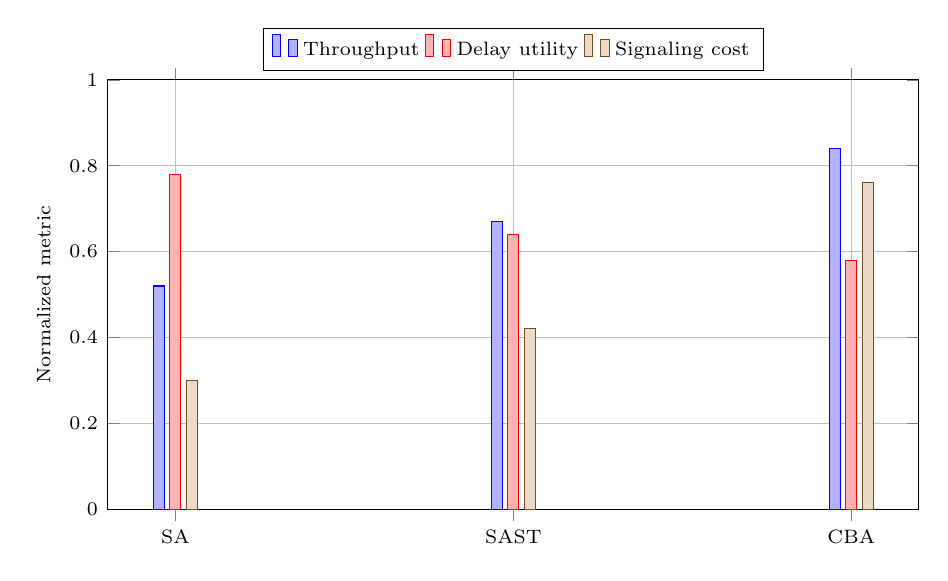
\begin{tikzpicture}
\begin{axis}[
  ybar,
  bar width=4pt,
  width=0.98\columnwidth,
  height=0.58\columnwidth,
  ymin=0, ymax=1.0,
  ylabel={Normalized metric},
  symbolic x coords={SA,SAST,CBA},
  xtick=data,
  legend style={font=\scriptsize, at={(0.5,1.02)}, anchor=south, legend columns=3},
  grid=both,
  tick label style={font=\scriptsize},
  label style={font=\scriptsize}
]
\addplot coordinates {(SA,0.52) (SAST,0.67) (CBA,0.84)};
\addplot coordinates {(SA,0.78) (SAST,0.64) (CBA,0.58)};
\addplot coordinates {(SA,0.30) (SAST,0.42) (CBA,0.76)};
\legend{Throughput,Delay utility,Signaling cost}
\end{axis}
\end{tikzpicture}
